\documentclass{beamer}
%\usepackage{colortbl}
\usepackage[latin1]{inputenc}
\usepackage{comment}
%\usetheme{Warsaw}
\usetheme{Frankfurt}
% \usecolortheme{dove}
\usepackage[absolute,overlay]{textpos} 
\usepackage{booktabs}
\usepackage{color}
\usepackage{threeparttable}
\usepackage{multirow}
\usepackage{rotating}

%\usepackage[table]{xcolor}
%\definecolor{tableShade}{HTML}{F1F5FA}



\title[Epistasis in expression]{Detection and replication of epistasis influencing human transcription}

\author{Gibran Hemani \and
Konstantin Shakhbazov \and \\
Grant W Montgomery \and
Peter M Visscher \and
Joseph E Powell}

\institute{Queensland Brain Institute, University of Queensland \and 
University of Queensland Diamantina Institute}

\date{}

\begin{document}

\AtBeginSection[]
{
  \begin{frame}<beamer>
    \frametitle{Outline}
    \tableofcontents[currentsection,currentsubsection]
  \end{frame}
}

\begin{frame}
\titlepage
\end{frame}


\section{Epistasis}
\subsection{}


\begin{frame}{Epistasis}
	\begin{definition}
		The effect on the phenotype caused by locus A depends on the genotype at locus B
	\end{definition}
\end{frame}


\begin{frame}{Two dimensional GWAS}
	\begin{center}
		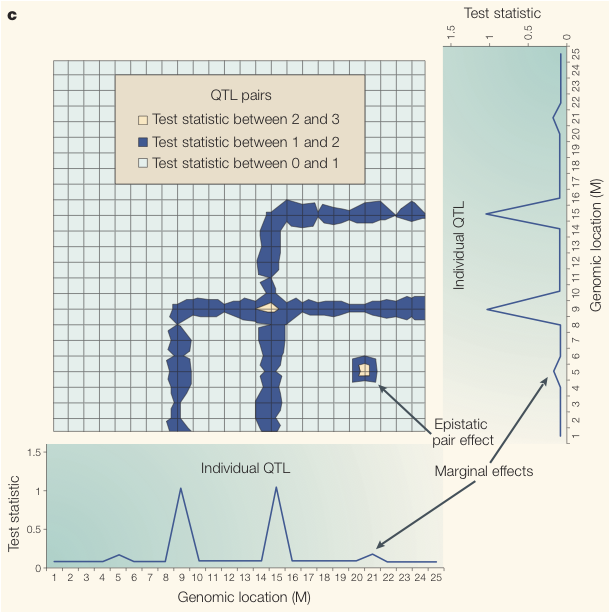
\includegraphics[width=7cm]{2dscan.png} \\
		{\tiny Carlborg 2004}
	\end{center}
\end{frame}


\begin{frame}{Impact of LD on detecting epistasis}
	\begin{center}
		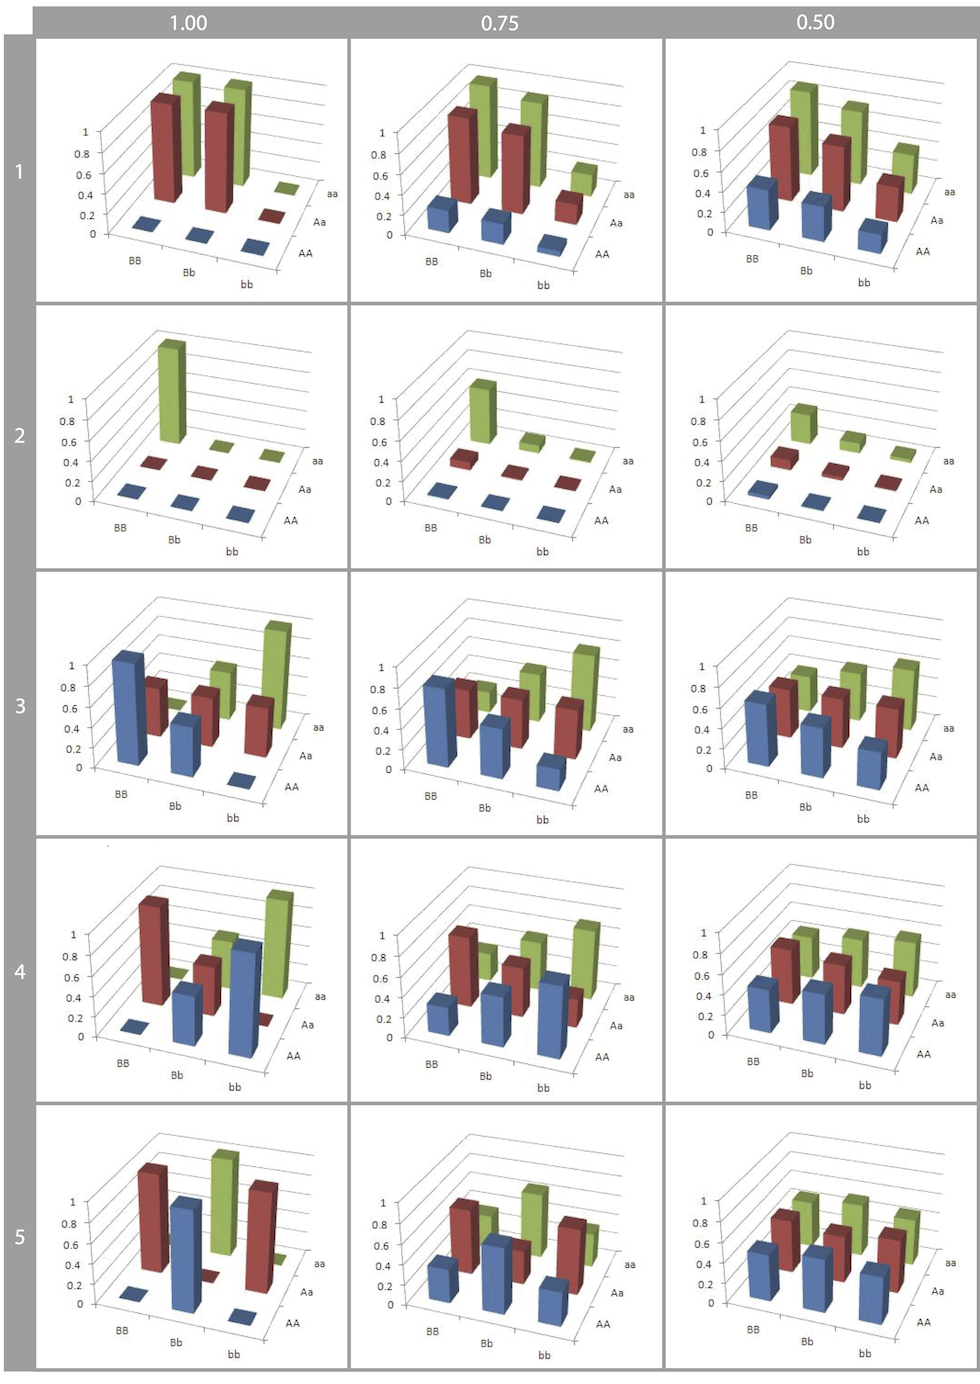
\includegraphics[width=5cm]{gpmaps_ld.png} \\
	\end{center}
\end{frame}


\begin{frame}{Multiple testing problem}
	\begin{block}{Curse of dimensionality}
		As the dimensionality of the search increases the background noise drowns out all real biological signals
	\end{block}

	\begin{equation}
		N_{\textrm{tests}} = \frac{m \times (m - 1)}{2} \nonumber
	\end{equation}
	\emph{e.g.} $500000k$ SNPs $\rightarrow 1.25 \times 10^{11}$ tests
\end{frame}


\section{Study design}
\subsection{}


\begin{frame}{Expression traits likely have larger effect sizes}
	\begin{center}
		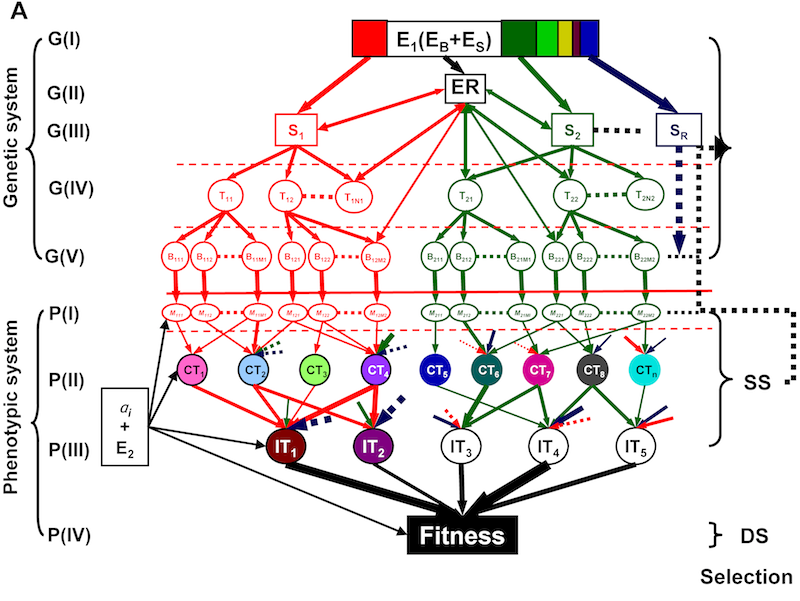
\includegraphics[width=7cm]{broadgp}
	\end{center}
\end{frame}


\begin{frame}{Discovery data}
	\begin{itemize}
		\item BSGS data - 842 individuals
		\item Gene expression on whole blood
		\item 7339 traits with $n \geq 90\%$
		\item 528,509 SNPs
	\end{itemize}
\end{frame}


\begin{frame}{Replication data}
	\begin{itemize}
		\item Fehrmann
		\begin{itemize}
			\item $n = 1240$
			\item Identical SNP chip and expression chip
		\end{itemize}
		\item EGCUT
		\begin{itemize}
			\item $n = 891$
			\item Identical SNP chip and expression chip
		\end{itemize}
		\item CHDWB
		\begin{itemize}
			\item $n = 139$
			\item Different SNP chip, same expression chip
		\end{itemize}
	\end{itemize}
\end{frame}


\begin{frame}{Computation}
	\begin{block}{Total number of tests}
		528,509 pairwise SNPs $\times$ 7,339 traits $=$ 1.02 quadrillion tests
	\end{block}
	\begin{block}{epiGPU software}
		Performs $\sim$12 million association tests per second
	\end{block}
	\begin{block}{GPU clusters}
		Supercomputers with 10s or 100s of GPUs can do this in a few weeks
	\end{block}
\end{frame}


\begin{frame}{Analysis outline}
	\begin{enumerate}
		\item Discovery scan
		\item Filtering of results based on threshold etc
		\item Filtering based on interaction vs genetic effects
		\item Replication in independent samples
	\end{enumerate}
\end{frame}


\begin{frame}{Discovery and filtering}
	\begin{block}{}
		Perform 8 d.f. test for full genetic effect (additive + dominance + epistasis) at each SNP pair
	\end{block}
	\begin{enumerate}
		\item Significance threshold $T = 2.91 \times 10^{-16}$
		\item Remove SNP pairs with any class size $< 5$
		\item Remove SNP pairs with LD $r^2 > 0.1$ or $D' > 0.1$
		\item Keep the sentinel SNP pair for each chromosome $\times$ chromosome $\times$ trait
		\item 11155 SNP pairs remain
		\item Perform nested test of full genetic model (8 d.f.) vs marginal model (a + d, 4 d.f.)
		\item Keep 4 d.f. interaction effects with $p < 0.05 / 11155$
	\end{enumerate}
	\begin{block}{}
		501 significant interaction SNP pairs
	\end{block}
\end{frame}


\section{Results}
\subsection{}

\begin{frame}{501 significant interactions in 238 expression traits}
	\begin{block}{Genomic positions}
		\begin{itemize}
			\item 47 \emph{cis}-\emph{cis}
			\item 441 \emph{cis}-\emph{trans}
			\item 13 \emph{trans}-\emph{trans}
		\end{itemize}
	\end{block}
	\pause
	\begin{block}{Marginal effects ($p < 1.0 \times 10^{-10}$)}
		\begin{itemize}
			\item 9 between two main effects
			\item 428 with only one main effect
			\item 64 with no main effects
		\end{itemize}
	\end{block}
	\pause
	\begin{block}{Largest epistatic variance component}
		\begin{itemize}
			\item 120 A x A
			\item 255 A x D
			\item 126 D x D
		\end{itemize}
	\end{block}
\end{frame}


\begin{frame}{Replication}
	\begin{itemize}
		\item Only 20 SNP pairs passed filtering in CHDWB
		\item 434 SNPs pairs passed QC in both EGCUT and Fehrmann
		\item 30 were significant for interaction $p$-values ($p < 0.05/434$) in EGCUT and Fehrmann
	\end{itemize}
\end{frame}


% q-q plots
\begin{frame}{Q-Q plots of replication interaction $p$-values}
	\begin{center}
		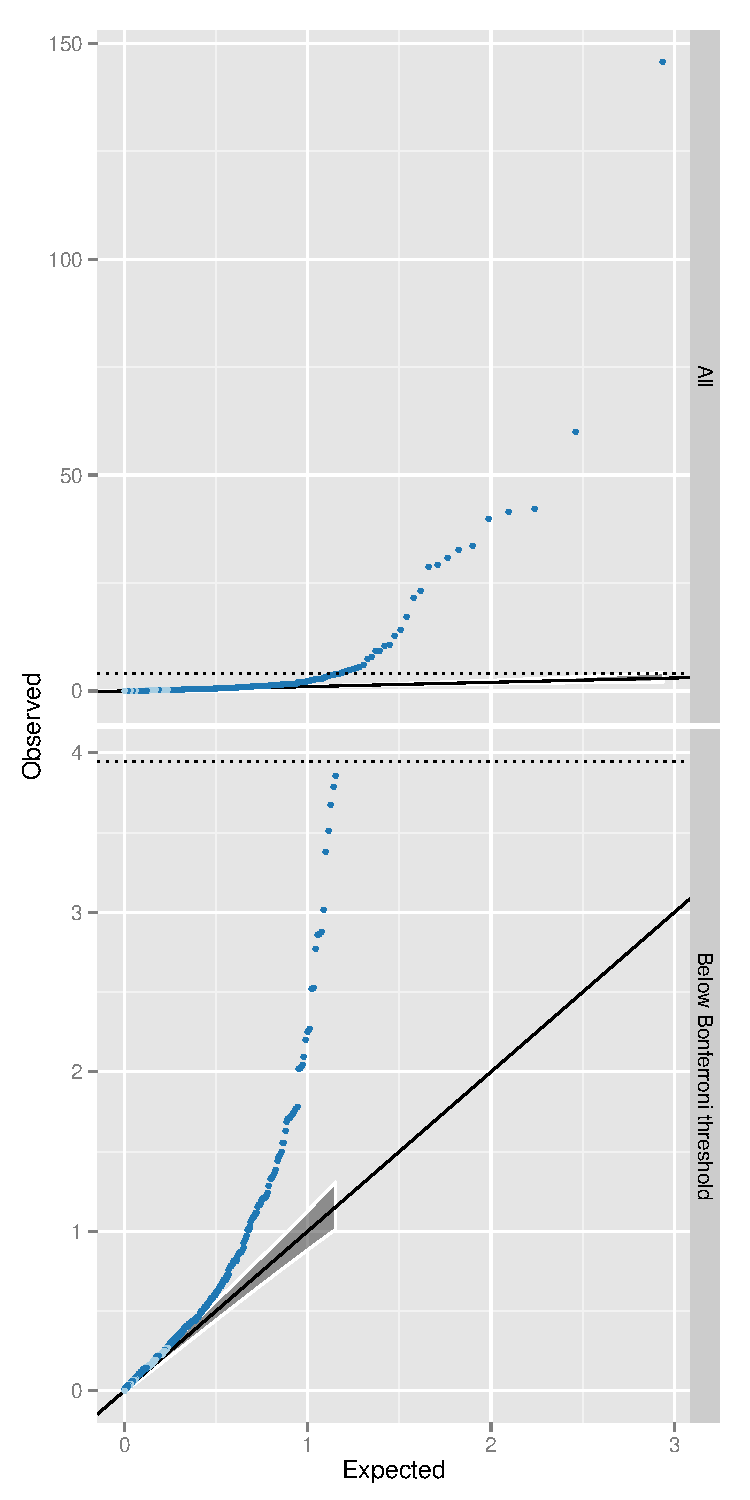
\includegraphics[height=7cm]{qqMeta}
	\end{center}
\end{frame}


\begin{frame}{Bonferroni level replicated GP maps}
	\begin{center}
		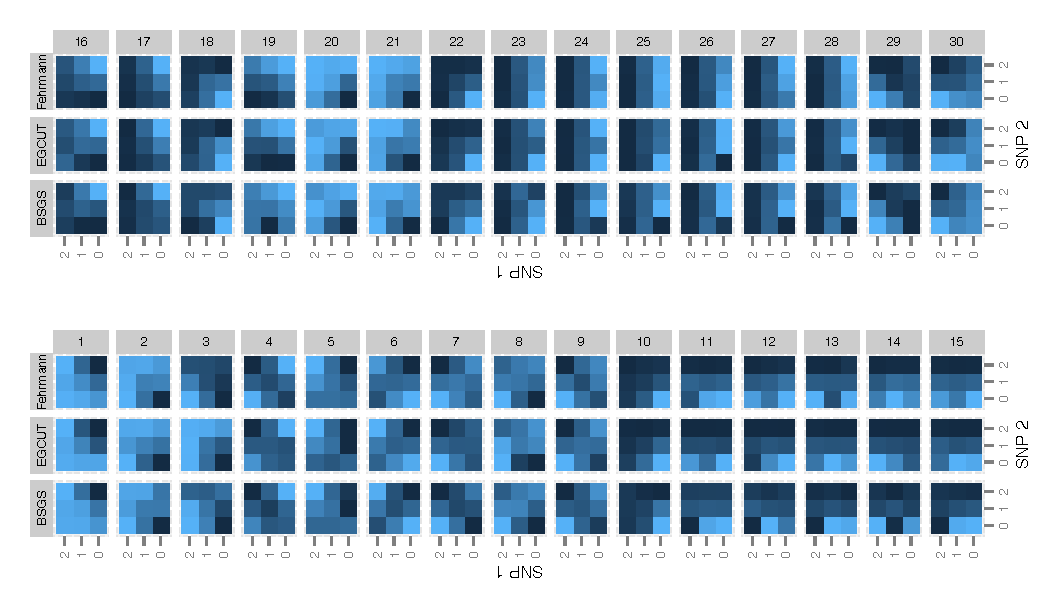
\includegraphics[width=11cm]{gpBonfRep}
	\end{center}
\end{frame}


\begin{frame}{Map of interactions}
	\begin{center}
		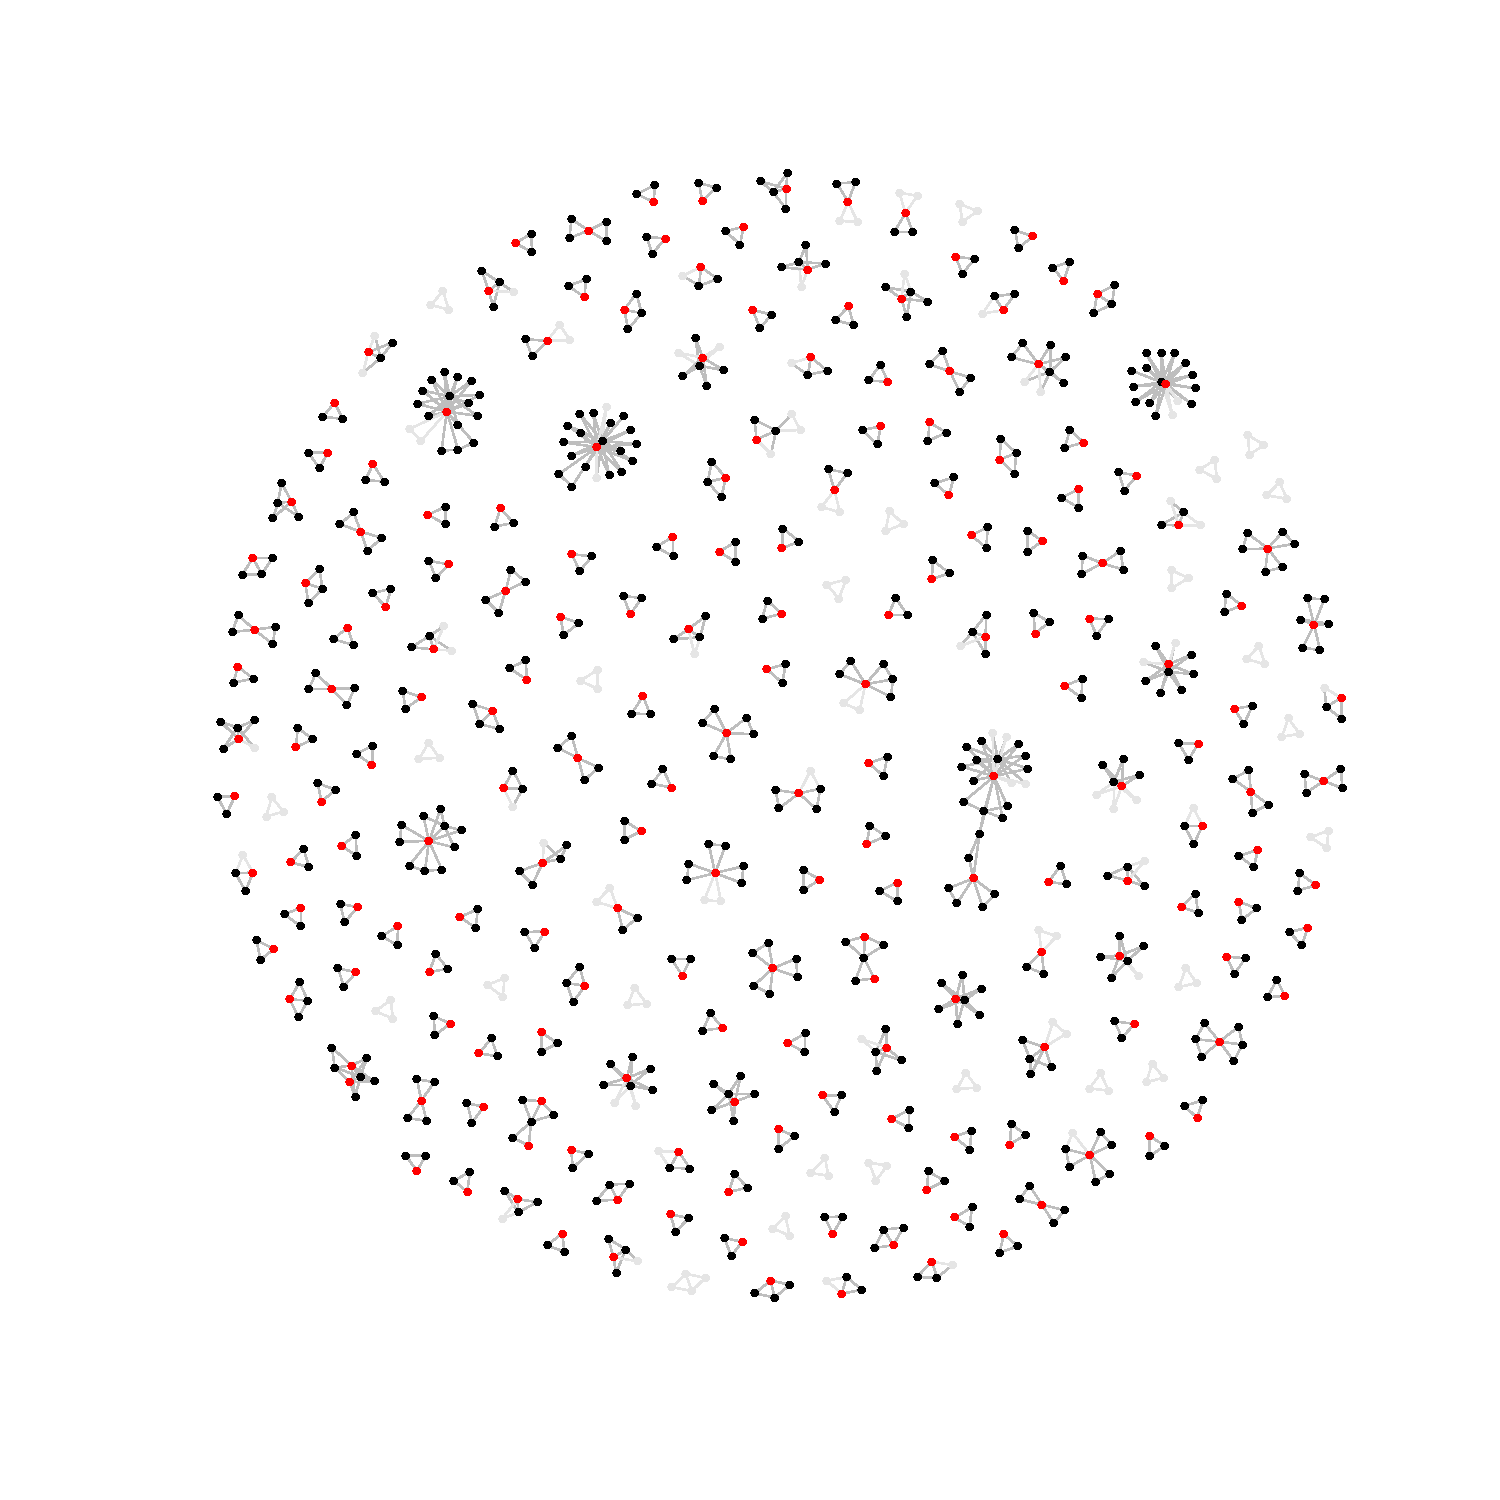
\includegraphics[height=7.5cm]{pale_gray_graph_of_interactions_2_lists}
	\end{center}
\end{frame}


\begin{frame}{TMEM149}
	\begin{center}
		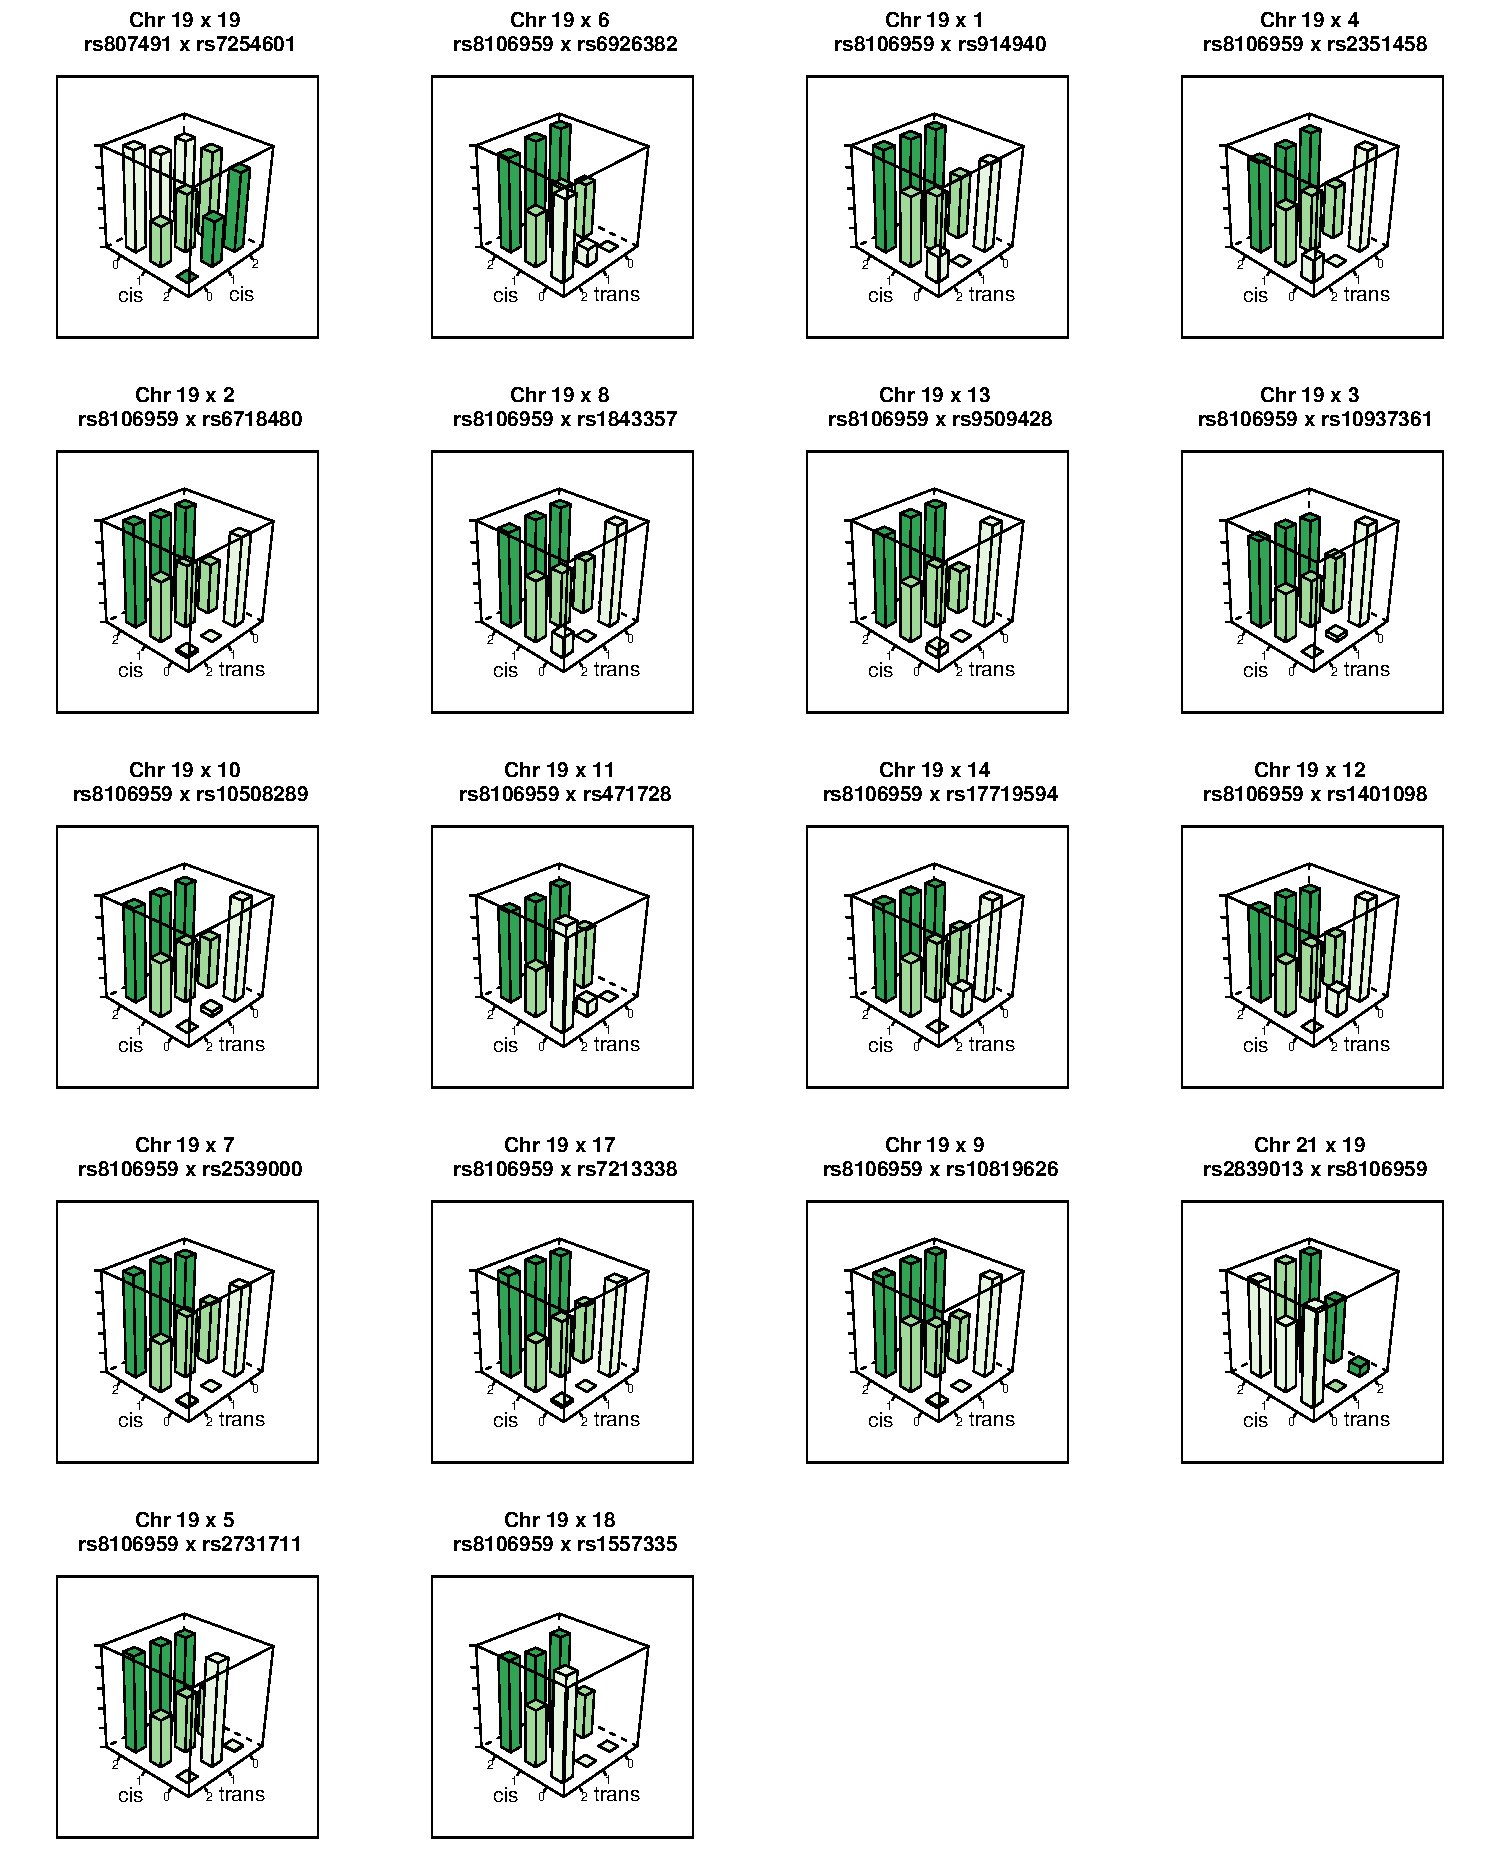
\includegraphics[height=7.5cm]{TMEM149_3d}
	\end{center}
\end{frame}


\begin{frame}{Chromosome interactions}
	\begin{center}
		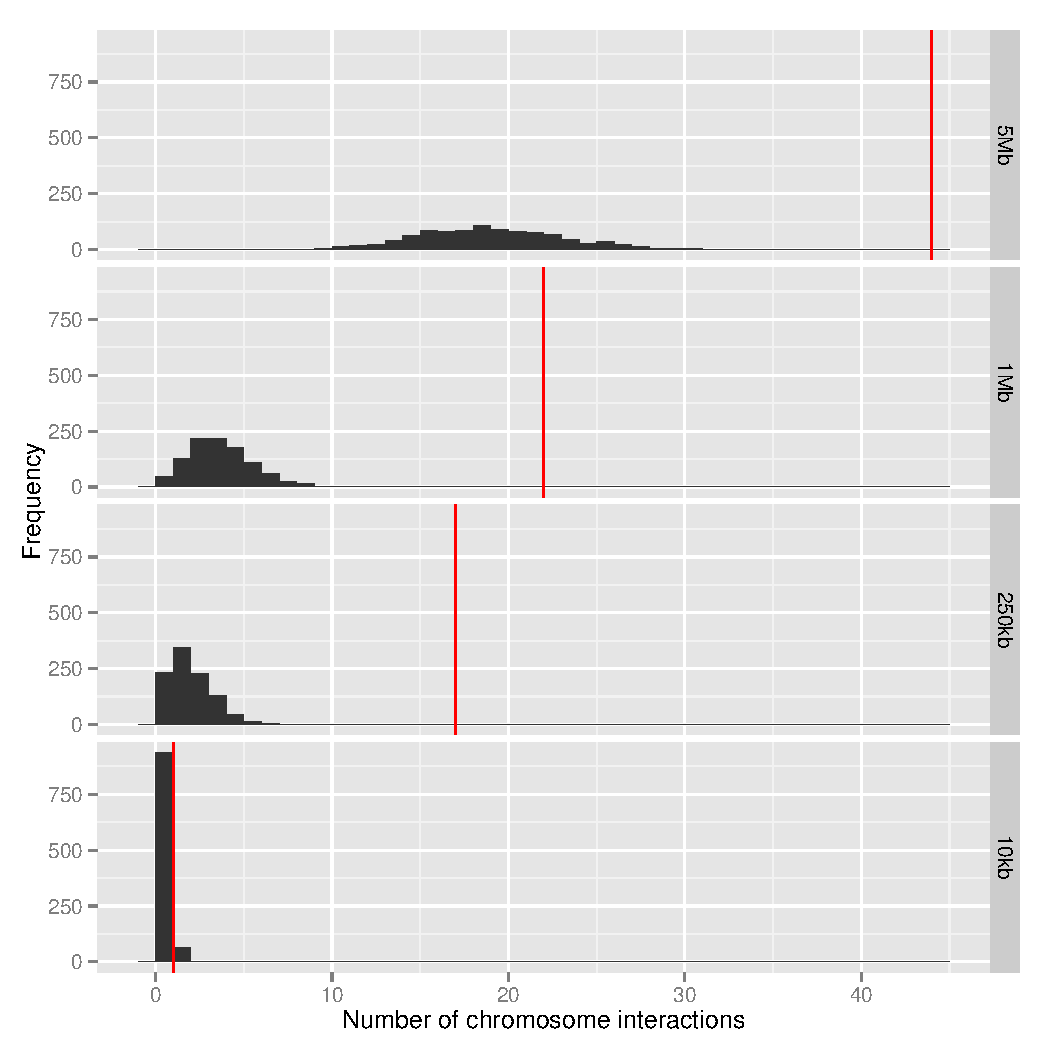
\includegraphics[height=7cm]{chromosome_interactions}
	\end{center}
\end{frame}


\begin{frame}{Contribution relative to additive effects}
	\begin{block}{At the same threshold ($2.91 \times 10^{-16}$)}
		\begin{itemize}
			\item 453 expression traits have a significant additive effect
			\item 238 have a significant interaction effect
		\end{itemize}
	\end{block}
	\pause
	\begin{block}{At the same threshold ($2.91 \times 10^{-16}$)}
		\begin{itemize}
			\item Significant additive effects explain 1.73\% of phenotypic variance of 7339 traits
			\item Significant epistatic effects explain 0.25\% (seven times less)
		\end{itemize}
	\end{block}
\end{frame}


\section{Acknowledgements}
\subsection{}


\begin{frame}{Acknowledgements}
	\begin{columns}[c]
		\column{0.5\textwidth}
			\begin{itemize}
				\item University of Queensland
				\begin{itemize}
					\item Joseph Powell
					\item Konstantin Shakhbazov
					\item Allan McRae
					\item Jian Yang
					\item Peter Visscher
				\end{itemize}
				\item QIMR
				\begin{itemize}
					\item Grant Montgomery
					\item Nicholas Martin
					\item Anjali Henders
				\end{itemize}
				\item Estonian Genomics Centre
				\begin{itemize}
					\item Tonu Esko
					\item Andres Metspalu
				\end{itemize}
			\end{itemize}
		\column{0.5\textwidth}
			\begin{itemize}
				\item Georgia Tech University
				\begin{itemize}
					\item Greg Gibson
				\end{itemize}
				\item University of Groningen
				\begin{itemize}
					\item Harm-Jan Westra
					\item Lude Franke
				\end{itemize}
				\item Computer resources
				\begin{itemize}
					\item iVEC at University of Western Australia
					\item MASSIVE project
					\item QBI IT Team
				\end{itemize}
			\end{itemize}
	\end{columns}
\end{frame}



\end{document}
